\documentclass[letterpaper, 11 pt, conference]{article}
\usepackage{setspace}
\usepackage{listings}
\usepackage{color}
\usepackage{float}
\usepackage{graphicx}

\usepackage[utf8]{inputenc}
\usepackage[english]{babel}


\usepackage[english]{babel}


\usepackage[letterpaper,top=2cm,bottom=2cm,left=3cm,right=3cm,marginparwidth=1.75cm]{geometry}


\usepackage{amsmath}
\usepackage{graphicx}
\usepackage[colorlinks=true, allcolors=blue]{hyperref}
\title{An Analysis of the Impact of Communal Attributes on Violent Crime in American Cities}
\author{Vedant Apte, Tien Ly, Annmarie Adams, Loren Aguilar, Hengze Ye, Dongyu Chen, Matthew Boentoro, Anqi Liu}

\begin{document}
\maketitle

\begin{abstract}
Using a unique data set linking the per capita violent crimes variable, population and the sum of crime variables considered violent crimes in the United States for 1994 instances from socio-economic data from the 1990 US Census, law enforcement data from the 1990 US LEMAS survey, and crime data from the 1995 FBI UCR, we estimate the impact of community on crime rates. Several models suggest that omitted variables related to multiple attributes do not bias the predictions.
\end{abstract}

\section{Introduction}

Over the last several decades in American society, a period that has witnessed many great advances in all facets of life, the existence of violent crime has consistently plagued the nation. However, a continuous effort over the last 25 years to reduce violent crime in the United States has seen the violent crime rate decrease sharply. That being said, crime rates vary significantly between the states, with states with such as Alaska, New Mexico, and Tennessee experiencing much higher crime rates than states such as Maine, New Hampshire, and Vermont in modern American society.
\\
\\This variance in crime rates across different communities has engendered the debate of whether or not attributes specific to a community cause or prevent more crime. One side of this debate argues that various issues related to community backgrounds leads to a volatility in the absolute number of criminals, or the number of current criminals becoming active. For example, some conditions such as low income and the number of single parent homes play a role in encouraging criminals who are inclined to commit crimes to do so, and furthermore, commit them in a violent manner. The other side of the debate argues that communities and their unique properties have little to do with crime, because individuals, not their surrounding environments, are responsible for the decisions (good and bad) that they make.
\\
\\The empirical research on this topic presents mixed results. This contradiction is likely due to a lack of credible and accessible data on community backgrounds in the United States. Many researchers use different sources and proxies when making connections involving community attributes, because the data can vary according to different sources. For instance, when talking about the gun ownership rate in communities, the General Social Survey, the suicide rates by firearm (Moody and Marvell), and the circulation of gun magazines (Duggan 2001) all have been used as attempted proxies for gun ownership. It is difficult to say how well these truly estimate the gun ownership rate.
\\
\\To make definitive statements about the impact that community attributes have on the violent crime rate in a society, further research must be done. The conclusions drawn from this research are important not only for the general public's understanding, but also for policymakers at the local, state, and federal levels. By taking a prospective approach to the problem and analyzing the impact of certain communal attributes on future violent crime rates, the aforementioned governments can produce educated legislation and courses of action that prevent the crime rate from rising in the first place, resulting in a safer America. Our project intends to analyze the \href{https://archive.ics.uci.edu/ml/datasets/Communities+and+Crime} {Communities and Crime Data Set} data set, found at the UC Irvine Machine Learning Repository, to draw these very conclusions by identifying numerical relationships between specific communal attributes and violent crimes per 100K. We will use this data set to train a machine learning model that can predict a normalized value for the violent crime per 100K given normalized inputs from one (or all) of three different categories: family, race, and wealth. To obtain data to draw our conclusions, we will construct both a regression model as well as a neural network model, as all of our inputs and our output are continuous, numeric attributes. The following sections of this paper will elaborate on our choice of input attributes, analyze our approach when developing and choosing between the two aforementioned predictive machine learning models, present our results and data (graphical and numerical), and identify potential errors along with future courses of action.

\section{Literature Review}
This review involves a number of interrelated discourses, including government records of crimes according to geological ranges, work on criminal reform and reduction on community level, and community studies on solutions towards these community issues. The following review simply highlights some of the recent relevant scholarly literature.
\\
\\First, some research in the field of crime variability among geological range studies has examined corrections. For regional comparisons in \cite{greenwade93}, the FBI divides the United States into four regions: Northeast, Midwest, South, and West. For 2019, the region with the lowest violent crime rate was the Northeast, with a rate of 292.4 per 100,000 residents, while the region with the highest violent crime rate was the West, with a rate of 413.5 per 100,000. For 2019, the region with the lowest property crime rate was the Northeast, with a rate of 1,350.4 per 100,000 residents, while the region with the highest property crime rate was the West, with a rate of 2,411.7 per 100,000. According to \cite{ref1}, the importance of communities is significant for social stability. As it says, in a city of 100,000, each new nonprofit community organization lead to a 1.2 percent drop in the homicide rate, a 1 percent reduction in the violent crime rate, and a 0.7 percent reduction in the property crime rate.
\\
\\Also, there are multiple materials that discuss the impact from community backgrounds on crime rates. In this citation \cite{ref5}, Brown describes the notion of penal spectator ship. She states, “many American citizens access punishment through cultural practices removed from formal institutions like prisons in a manner which, although largely unacknowledged, massively extends throughout our social foundations” (p4). Brown is interested in studying “penal subjectivity,”which involves “performances of punishment, when distant from actual punishment” (p5). Brown states, “citizens may participate vicariously in mediated worlds when pain is inflicted across television, films, recreation and news. They may be disturbed by these images. They may find such engagement titillating” (p5). 
\\
\\Furthermore, more and more importance are put on the impact of communities on crime and researchers are looking for ways of regulating community to reduce crime rate. For instance, in \cite{ref2}, p233, "a theory of street lighting focusing on its role in increasing community pride and informal social control may be more plausible than a theory focusing on increased surveillance and increased deterrence." This implies reflecting the good angle of communities on reducing crime rate. Similar material is in \cite{ref4}, which includes impacts of poverty alleviation on crime. No doubt that workforce development and substance abuse prevention are two sure-fire ways to “feed two birds with one seed” by reducing both poverty and crime. 
\\
\section{Data Set Description}
\\
\\Our data set contains 128 different attributes: 122 of these are predictive, 5 are non-predictive, and 1 is the output. Of the 122 predictive inputs, many inputs did not have data present (either due to unavailability of data or failure to collect). After removing these data columns from the data set, we were able to identify six general categories that encompassed the remaining attributes: biographical information attributes, family attributes, race attributes, wealth attributes, housing condition attributes, and education attributes. Upon creation of a heat map with all of these input attributes, we identified the attributes from each category with the highest correlation with our desired output, violent crimes per 100K. We were able to select eight different input attributes from three of the six categories above to use as inputs into our machine learning model. The attributes from the biographical information, housing condition, and education categories did not have a high enough correlation to be suitable to use in our models. Here are the input attributes that we decided to proceed with for our models:
\\
\\Race:
\\racepctblack: percentage of population that is African American
\\racePctWhite: percentage of population that is white
\\
\\Family:
\\PctKids2Par: percentage of kids in family housing with two parents
\\TotalPctDiv: percentage of population that is divorced
\\PctIlleg: percentage of kids born to individuals that never married
\\
\\Wealth:
\\PctPopUnderPov: percentage of population that is under the poverty level
\\pctWPubAsst: percentage of population with public assistance income
\\pctWInvInc: percentage of population with investment income
\\
\\Figure 1 below is a heat map with the correlation values between each of the input attributes described above, and the output variable, violent crimes per 100K.
\begin{figure}[H]
\centering
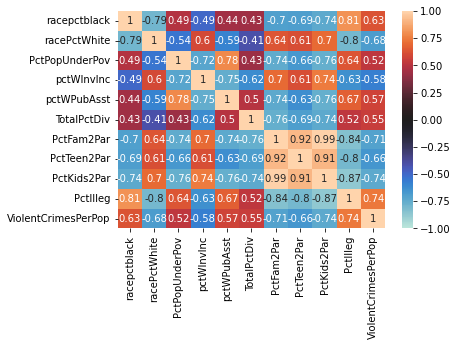
\includegraphics[width=10cm]{hotbox.png}
\caption{The heat map for our attributes.}
\label{fig:hotbo}
\end{figure}
From the hot spot of our data set, we chose to include both of the following (Set A):
\\
\\racepctblack: 0.63
\\racepctwhite: -0.68
\\
\\and three out of the following (Set B):
\\
\\PctKids2Par: -0.74
\\TotalPctDiv: 0.55
\\PctIlleg: 0.74
\\
\\and also three out of the following (Set C):
\\
\\PctPopUnderPov: 0,52
\\pctWPubAsst: 0.57
\\pctWInvInc: -0.58
\\
\\The first two attributes (Set A) indicate that in cities in which there is a higher black population, there is a relatively strong positive correlation with the output attribute, violent crimes per 100K people. Similarly, we can say the same for cities with a higher white population (except it has a relatively strong negative correlation). No racism intended with these two statements, just analyzing the data. 
\\
\\Also, about family (set B), we picked the most related age range -- PctKids2Par (-0.74), which is more related than PctTeen2Par and PctFam2Par -- together with the TotalPctDiv and PctIlleg. The percentage of population that is divorced and percentage of kids born to individuals that never married are both typical aspects that could show the incompleteness of family that we wanna discuss. 
\\
\\For wealth (set C), we chose all three related attributes as well.Population under the poverty level should be the most explicit viewpoint to show the lower bound of a community's wealth condition, while population with public assistance income could be a good supplement towards this. In addition, population with investment income could show the upper bound of the wealth of a community, which could also be a typical attribute.
\\
\\Additionally, 
\href{https://www.census.gov/prod/1/statbrief/sb93_2.pdf}{this link} provides a nice graphic on the first page, which demonstrates that leading up to the 1990s (which is when the data from our data set was collected), the number of African American homes with two parents was decreasing every year. This lines up with the correlation values from the attributes above. Let's explore this:
\\
\\When the number of families with less than 2 parents in the household is high, there is a strong positive correlation ($>$0.7) with more violent crime per 100K. The link tells us that there was a large percentage of African American families with less than 2 parents in the household in the 1990s. The racepctblack attribute gives a positive correlation with violent crimes per 100K. This means that a high racepctblack and high PctFam2Par: -0.71 should give a high violent crimes per 100K. Likewise, a low racepctblack, high racepctwhite, and low PctFam2Par should give a low violent crimes per 100K.
\\
\\We can use two out of the four attributes from the second set (Set B), to possibly make this connection with the first set of attributes (Set A).

\section{Algorithm Design}
 
\begin{figure}[H]
\centering
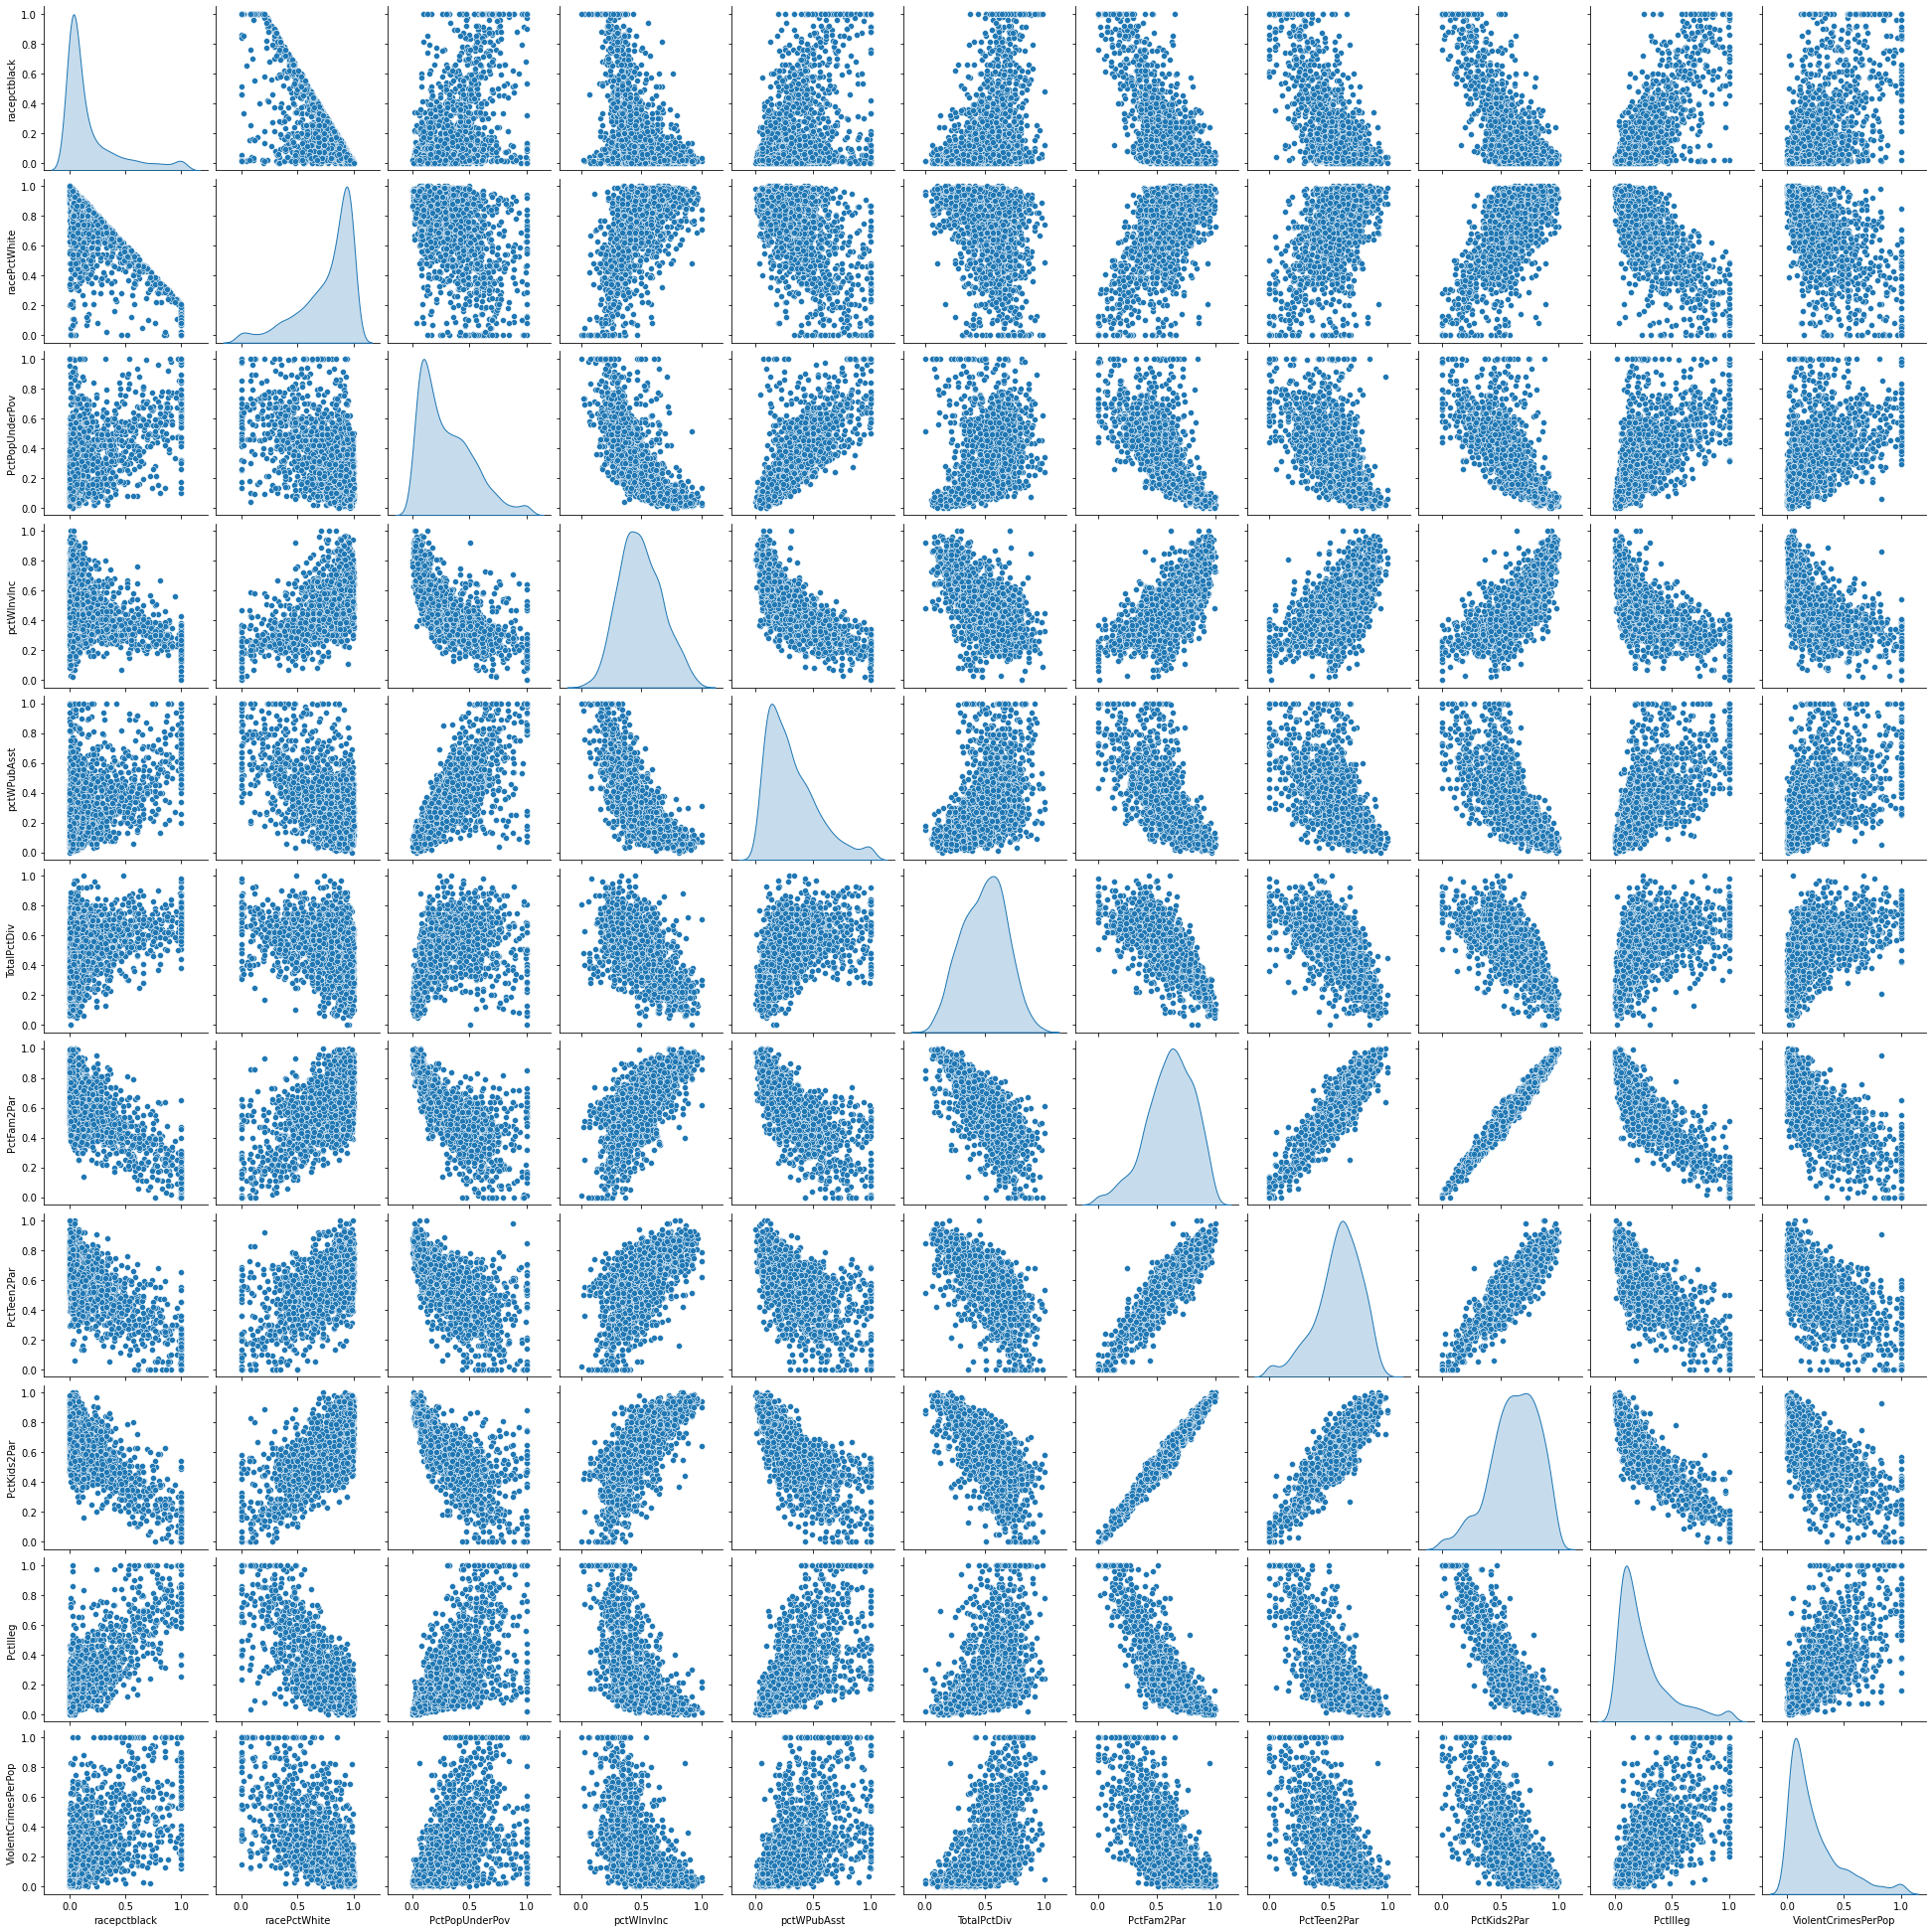
\includegraphics[width=0.4\textwidth]{pairplot.png}
\caption{\label{fig:pairplot}The pair plot for our attributes.}
\end{figure}
From the pair plot, it can be found out that the data set has high linearity, meaning that polynomial regression may not function as efficiently as simple linear regression. Thus, we will abandon polynomial regression and choose linear regression and artificial neural networks.

\subsection{Linear Models}
For our first part, we implied the linear regression. The data set is all numerical and our pair plot already shows that the high linearity of crime rate and thee attributes we want to discuss. To compare the affects of different attributes we made various inputs, including family, wealth, race and all these three attributes together. The mean-square errors (MSEs) are calculated to quantify the accuracy.
\\
\\Also, to increase accuracy, we used k-fold Cross Validation with n\_splits = 10 to generalize our linear model. We calculated the MSEs of the 10 folds and took an average.


\subsection{NN Models}
Meanwhile, although the linear regression should preform well based on our prediction, other methods were also required. That is because our attributes could not be completely linear based on our experience in daily life. However, polynomial regression may not be a better and more efficient choice due to the pair plot graph. As a result, in order to reduce the errors and bias, we need methods that could deal with the data on a higher level with more accuracy.
\\
\\Thus, we also attempted a neural network model with three hidden layers. Each node has a relu activation. The nodes of these layers are 40, 10 and 4. The learning rate was 0.01, in that we hoped to generalize an accuracy model.
\\
\\To increase accuracy, we also used a 10-split k-fold Cross Validation for generalization with an averaged MSE.





\section{Experiment Results}


\subsection{Comparison of different models}
Below is the our four linear models with different inputs and their MSEs accordingly.
\begin{table}[H]
\centering
\begin{tabular}{ |c|p{2cm}|p{8cm}|c| } 
Model number & {Comparison Type vs. Violent Crimes Per 100K} &Input Attributes & MSE \\\hline
Model 1 & Family   & {PctKids2Par, PctIlleg, TotalPctDiv} & 0.019800573421352132
\\
Model 2 & Wealth  & PctPopUnderPov, pctWPubAsst, pctWInvInc & 0.030321798734355372
\\Model 3 & Race  & racepctblack, racePctWhite & 0.02548976923588889
\\Model 4 & All Attributes From Above  & PctKids2Par,  PctIlleg,  TotalPctDiv,  PctPopUnderPov,  pctWPubAsst,  pctWInv, racepctblack, racePctWhite & 0.018916681213162385
\\
\end{tabular}
\caption{\label{tab:widgets}Linear models table.}
\end{table}
It could be figured out that each model has relatively high accuracy in predicting the crime. Notice that different attributes might lead to different prediction accuracy. For single attribute, completeness of family could most precisely predict crime. And in general, with input of more attributes the accuracy is also increased. Note that this could also partially reflect that these attributes are not completely independent: an incomplete family might be more likely to , and the imbalance retreat on different races can also lead to inequality of social positions, thus affecting income and wealth. 
\\
\\The prediction graph trained from all attributes, compared with the actual values, is shown below.
\begin{figure}[H]
\centering
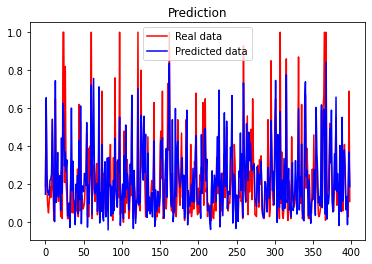
\includegraphics[width=8cm]{pred_all.png}
\caption{The prediction of linear model with all attributes.}
\label{fig:hotbo}
\end{figure}
\hspace*{\fill} 
\\
We can see that in general the prediction could fit the test, but in condition where crime rate in higher than 0.8 the prediction usually could not get that high and failed to precisely fit. It is not a serious problem as it avoided to be overfilling.
\\
\\And the following is the k-fold table for our most accurate linear model, with which we can get that our generalized MSE was around  0.021.
\begin{table}[H]
\centering
\begin{tabular}{ |c|c| } 
Model number & MSE \\\hline
1& 0.024421074129946138
\\2&0.021957326289128574
\\3&0.02964691696703562
\\4&0.02223141399406684
\\5& 0.019892430104690103
\\6& 0.017386771876898813
\\7&: 0.019961261543826495
\\8& 0.015644956122021755
\\9& 0.01933080762206681
\\10&0.019963008823498555
\\Overall & 0.021043596747317976
\end{tabular}
\caption{\label{tab:widgets}K-Fold table for linear model.}
\end{table}
\hspace*{\fill} 
\\Meanwhile, the results of our ANN are generated with MSE as 0.017634989693760872. As a result,it appears that based on our data set, neural networks might function slightly better.
\\
\\Below is the prediction graph of neural network, it showed similar but smaller Incarnation compared to the linear model. 
\begin{figure}[H]
\centering
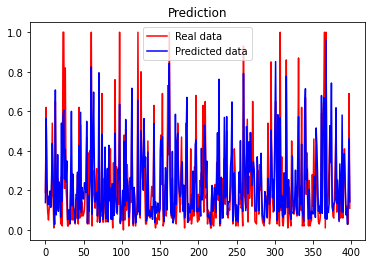
\includegraphics[width=8cm]{pred_nn.png}
\caption{The prediction of ANN model with all attributes.}
\label{fig:hotbo}
\end{figure}

Also, to generalize our result, we attempted k-Fold and here is its list.


\begin{table}[H]
\centering
\begin{tabular}{ |c|c| } 
Model number & MSE \\\hline
1& 0.02551523968577385
\\2&0.019871624186635017
\\3&0.024044839665293694
\\4&0.018758008256554604
\\5& 0.016902180388569832
\\6& 0.01307844277471304
\\7&: 0.016748927533626556
\\8& 0.013514549471437931
\\9& 0.014407705515623093
\\10& 0.01636567711830139
\\Overall & 0.0179207194596529
\end{tabular}
\caption{\label{tab:widgets}K-Fold table for ANN model.}
\end{table}
\hspace*{\fill} \\

To sum up, our two models, linear regression and ANN, all showed high accuracy in predicting the crime rate based on chosen community attributes. The neural network functioned slightly better, which is not surprising, as the whole data set was not completely linear, Based upon our findings, after discussion of some possible errors, we can make our solution accordingly. 


\subsection{Errors and Possible Improvement}
The prediction curves we found fits our curve pretty  well, but in each model, linear and ANN, for rate around 0 it overestimates and above 0.8 it underestimates. Something that was of interest was the spike in crime rates around 1. Upon further inquiry we found that there were 10 communities that had an extremely high crime rate of almost 1. Although it may be possible that the whole communities had crime records, this is most likely due to the way the researchers of our data set gathering these information; maybe they just recorded the criminals' data in some communities and thus making these communities "100\% criminal".
\\\\To remedy this issue, it will require researchers to redo the survey with more accurate work with a much larger amount,  which could be very hard depending on the researching condition.

\section{Conclusion and Discussion}
From our research, to reduce crime rates, improving the community circumstances is significant. Due to their high relation ship to crime rate, making family structure complete, reducing race distinguishing and increasing general social wealth could function well in stabilizing our social security. Several methods could be applied to improve this situation.
\\
\\One way to get there is to support community organizations. Our study provides empirical evidence for something community organizers have said for decades: crime reduction is difficult without addressing problems stemming from chronic poverty. These organizations play a significant role in reducing crime rates not by changing justice system policy but by providing more support for individuals without costing too much wealth of individuals. 
\\
\\Another is Federal legislation. For instance, the Reverse Mass Incarceration Act would provide resources to states to pursue creative approaches to helping communities bring down crime, while bills like the Sentencing Reform and Corrections Act would help fix our misguided use of overly-harsh punishments to reduce crime. While more research is needed to improve our public response to crime, supporting ad reforming the community to help drive the crime decline is an excellent place to start.
\\
\\Meanwhile, due to the slight accuracy error, possible improvement can still be made to the information gather methods on community attributes. In community research, the use of small group methods, used by the FBI, such as key informant surveys, community leader interviews, and focus and discussion groups could not function as well as before in today's America. Additional research is needed on the relative cost, value, and results of such techniques compared with traditional community survey methods.

\clearpage
\bibliographystyle{alpha}
\bibliography{sample}

\end{document}